\documentclass[12pt,a4paper]{article}
\usepackage[utf8]{inputenc}
\usepackage{polski}
\usepackage[polish]{babel}
\usepackage{amsmath}
\usepackage{amsfonts}
\usepackage{amssymb}
\usepackage{graphicx}
\usepackage{wrapfig}
\usepackage{caption}
\usepackage{mhchem}

\numberwithin{equation}{section}


\renewcommand{\baselinestretch}{1.5}
\captionsetup[figure]{labelformat={default},name={\bfseries Rys.}}
\captionsetup[table]{labelformat={default},name={\bfseries Tab.}}

\newcommand*{\captionsource}[2]{%
	\caption[{#1}]{%
		#1%
		\\\hspace{\linewidth}%
		\textbf{Żródło:} #2%
	}%
}


\title{4. Współczynnik załamania światła\\ dla ciał stałych}
\date{15 listopada 2017}	
\author{
	Zespół 3: Górski Paweł, Sozańska Ada\\
	EAIiIB Informatyka, Rok II
}

\begin{document}
\maketitle
% WPROWADZENIE
\section{Wprowadzenie}
Celem tego doświadczenia jest wyznaczenie wartości współczynnika załamania światła dla płytek wykonanych ze szkła i plexiglasu.

\subsection{Prawo załamania światła}

Prawo załamania światła mówi o tym, że jeżeli światło przechodzi z ośrodka $A$ do ośrodka $B$ o innych właściwościach optycznych, to stosunek sinusa kąta padania światła $\theta_A$ do sinusa kąta załamania światła $\theta_B$ jest stały. Stała ta nazywana jest współczynnikiem załamania światła i oznaczana przez $n$:
\begin{equation}
	n = \frac{\sin \theta_A}{\sin \theta_B}.
	\label{eq:n1}
\end{equation}

Współczynnik załamania światła jest inny dla różnych długości fali, co widoczne jest między innymi podczas zjawiska dyspersji w pryzmacie.

\subsection{Wyprowadzenie zależności}

Dla bardzo małych kątów $\alpha$ i $\beta$ na mocy twierdzenia Taylora zachodzi przybliżenie:
\begin{equation}
	\frac{\sin \alpha}{\sin \beta} \approx \frac{\alpha}{\beta} \approx \frac{\tan \alpha}{\tan \beta},
\end{equation}
co pozwala nam przekształcić równanie (\ref{eq:n1}) do postaci:
\begin{equation}
	n = \frac{\tan \alpha}{\tan \beta}.
\end{equation}

Jak widać na schemacie (Rys. \ref{fig:img1}) możemy w łatwy sposób podać zależności tangensa kątów od innych parametrów.


\begin{wrapfigure}{l}{0.4\textwidth}
	\centering
	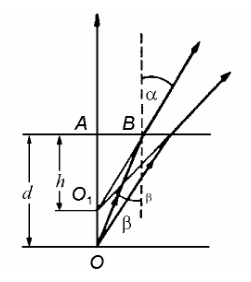
\includegraphics[width=0.3\textwidth]{img/swiatlo.png} 
	\captionsource{Bieg promieni podczas załamania światła}{Instrukcja dośw.\\}
	\label{fig:img1}
\end{wrapfigure}

Możemy zapisać, że:
\begin{equation}
	\tan \alpha = \frac{AB}{h},~~\tan \beta = \frac{AB}{d},
\end{equation}
gdzie $h$ jest odległością pozorną od obserwatora, a $d$ odległością rzeczywistą. W rezultacie otrzymujemy wzór:
\begin{equation}
	n = \frac{d}{h}.
	\label{eq:n2}
\end{equation}

Dla układu pomiarowego wykorzystanego w tym doświadczeniu (mikroskopu) możemy wykorzystać wzór (\ref{eq:n2}), ponieważ w rzeczywistości kąty $\alpha$ i $\beta$ są bardzo małe (patrzymy na płytkę prawie pod kątem prostym). W przypadku badania współczynnika załamania światła przy pomocy mikroskopu, $d$ będzie grubością rzeczywistą płytki. Grubość pozorną płytki $h$ będziemy mogli wyznaczyć dzięki dużemu przybliżeniu mikroskopu i jego wąskiemu zakresowi głębi ostrości, jako różnicę między górnym i dolnym poziomem płytki.

% WYKONANIE ĆWICZENIA
\section{Wykonanie ćwiczenia}
\label{sec:2}

W celu wykonania doświadczenia wykorzystaliśmy:
\begin{itemize}
	\item Mikroskop z czujnikiem mikrometrycznym i nasadką krzyżową,
	\item Śrubę mikrometryczną,
	\item Dwie płytki z plexiglasu o różnej grubości,
	\item Płytkę ze szkła.
\end{itemize}

Doświadczenie rozpoczęliśmy od zmierzenia grubości każdej z płytek za pomocą śruby mikrometrycznej o dokładności $0,01$~mm.

Następnie umieściliśmy każdą płytkę pod mikroskopem i wykonaliśmy po sześć pomiarów dla płytek z plexiglasu, a siedem pomiarów dla płytki szklanej. Na każdej z płytek namalowany został krzyżyk w taki sposób, że jedna linia znajdowała się na górnej powierzchni, a druga na spodzie płytki. Dla każdej linii dostosowywaliśmy ostrość, a następnie odczytywaliśmy pomiary z zegara mikrometrycznego o dokładności $0,01$~mm.

\pagebreak
% OPRACOWANIE DANYCH POMIAROWYCH
\section{Opracowanie danych pomiarowych}
\subsection{Analiza pomiarów dla plexiglasu}

W poniżej tabeli znajdują się dane pomiarowe dla płytek z plexiglasu:

\begin{table}[!ht]
	\caption{Wartości pomiaru dla płytek z plexiglasu}
	\centering
	\begin{tabular}{c|c|c||c|c|c}
		\hline \multicolumn{3}{c||}{Płytka 1: $d_1 = 3,80$~mm} & \multicolumn{3}{c}{Płytka 2: $d_2 = 4,93$~mm} \\ \hline 
		$a_d$~[mm] & $a_g$~[mm] & $h$~[mm] &  $a_d$~[mm] & $a_g$~[mm] & $h$~[mm] \\ \hline \hline
		$4,31$ & $1,80$ & $2,51$ & $3,94$ & $0,68$ & $3,26$\\
		$4,30$ & $1,80$ & $2,50$ & $3,94$ & $0,67$ & $3,27$\\
		$4,27$ & $1,81$ & $2,46$ & $3,93$ & $0,68$ & $3,25$\\
		$4,30$ & $1,80$ & $2,50$ & $3,94$ & $0,66$ & $3,28$\\
		$\textbf{4,26}$ & $\textbf{1,81}$ & $\textbf{2,45}$ & $3,92$ & $0,65$ & $3,27$\\
		$4,28$ & $1,80$ & $2,48$ & $\textbf{3,91}$ & $\textbf{0,67}$ & $\textbf{3,24}$\\ \hline
	\end{tabular}
	\label{tab:tab1}
\end{table}

Pogrubione dane zawarte w tabeli (Tab. \ref{tab:tab1}) zostały odrzucone ze względu na podejrzenie popełnienia błędu grubego podczas pomiaru.

Wyliczone średnie grubości pozorne oraz odpowiadające im niepewności pomiaru dla powyższych danych wynoszą kolejno:
\begin{equation}
	\begin{split}
		& h_1 = (2,4900 \pm 0,0089)~\textrm{mm}, \\
		& h_2 = (3,2660 \pm 0,0050)~\textrm{mm}.
	\end{split}
\end{equation}

Współczynniki załamania dla obu płytek wyznaczamy ze wzoru (\ref{eq:n2}), a niepewność pomiaru współczynnika ze wzoru poniżej:
\begin{equation}
	u(n) = n \sqrt{\Bigg(\frac{u(d)}{d}\Bigg)^2 + \Bigg(\frac{u(h)}{h}\Bigg)^2},
	\label{eq:un}
\end{equation}
będącego konsekwencją wzoru na niepewność względną pomiaru.

Dla powyższych płytek mamy:
\begin{equation}
	\begin{split}
		n_1 = 1,5261 \pm 0,0067, \\
		n_2 = 1,5095 \pm 0,0038.
	\end{split}
\end{equation}

Wartość tabelaryczna współczynnika załamania światła dla plexiglasu wynosi $n_0 = 1,492$.
\begin{equation}
	\begin{split}
		&|n_0 - n_1| = 0,034 ~> U(n_1) = 0,013, \\
		&|n_0 - n_2| = 0,0174 > U(n_2) = 0,0077.
	\end{split}
\end{equation}
Stwierdzamy, że wyniki dla obu płytek nie są zgodne z wartością tabelaryczną.

Następnie sprawdzimy zgodność obu pomiarów ze sobą, dzięki czemu będziemy mogli stwierdzić, czy współczynnik załamania światła $n$ jest niezależny od grubości płytki.
\begin{equation}
	|n_1 - n_2| = 0,016 > 2 \cdot \sqrt{u(n_1)^2 + u(n_2)^2} = 0,015.
\end{equation}
Jak widać powyżej, wyniki nie są ze sobą zgodne w granicach błędu.

\subsection{Analiza pomiarów dla szkła}

W poniżej tabeli znajdują się dane pomiarowe dla szklanej płytki:

\begin{table}[!ht]
	\caption{Wartości pomiaru dla szklanej płytki}
	\centering
	\begin{tabular}{c|c|c}
		\hline \multicolumn{3}{c}{Płytka: $d_1 = 2,18$~mm} \\ \hline 
		$a_d$~[mm] & $a_g$~[mm] & $h$~[mm] \\ \hline \hline
		$\textbf{4,80}$ & $\textbf{3,41}$ & $\textbf{1,39}$ \\
		$4,84$ & $3,38$ & $1,46$ \\
		$4,84$ & $3,41$ & $1,43$ \\
		$4,86$ & $3,41$ & $1,45$ \\
		$4,85$ & $3,39$ & $1,46$ \\
		$4,87$ & $3,39$ & $1,48$ \\
		$4,86$ & $3,40$ & $1,46$ \\ \hline
	\end{tabular}
	\label{tab:tab2}
\end{table}

Pogrubione dane zawarte w tabeli (Tab. \ref{tab:tab2}) zostały odrzucone ze względu na znacznie odbiegający od reszty wynik, który sugeruje popełnienie błędu grubego podczas pomiaru.

\pagebreak
Wyliczona średnia grubość pozorna oraz odpowiadająca jej niepewność pomiaru dla powyższych danych wynosi:
\begin{equation}
	h = (1,4567 \pm 0,0066)~\textrm{mm}.
\end{equation}

Współczynniki załamania dla obu płytek wyznaczamy ze wzoru (\ref{eq:n2}), a niepewność z wyznaczonego wyżej wzoru (\ref{eq:un}):

\begin{equation}
	n = 1,4966 \pm 0,0096.
\end{equation}

Wartość tabelaryczna współczynnika załamania światła dla szkła wynosi $n_0 = 1,50$.
\begin{equation}
	|n_0 - n| = 0,003 < U(n_1) = 0,019.
\end{equation}

Stwierdzamy, że wynik dla szklanej płytki jest zgodny z wartością tabelaryczną.

\section{Wnioski}

Wartości współczynnika załamania dla plexiglasu nie były zgodne z wartością tabelaryczną odpowiadającą temu materiałowi. Prawdopodobnie było to spowodowane popełnieniem błędu systematycznego przez eksperymentatorów, na przykład podczas dobierania ostrości mikroskopu przy pomiarze grubości pozornej. Dodatkowo zwiększenie ilości pomiarów mogłoby znacząco poprawić wynik tego doświadczenia.

Porównanie ze sobą wyników dla obu płytek nie pozwala nam stwierdzić niezależności współczynnika załamania światła od grubości ośrodka, ponieważ wyniki nie były ze sobą zgodne w granicy błędu.

Z kolei wartość współczynnika dla szkła okazała się zgodna z wartością tabelaryczną, z czego wynika, że dane dla tej płytki nie były obarczone błędami grubym bądź systematycznym.

\end{document}
